\chapter{Appendix}

\section{One data file per subject}

For behavioural data, it is common to save data from all subjects in a single file, with each row being a sample (subject or trial) and each column being a variable (or feature). PRoNTo however does not accept this format as multiple rows could arise from another input dimensionality of the data that the user wishes to keep (e.g. 2D connectivity matrix instead of vectorized).
\\

We hence provide a script that transform a \#samples x \#features matrix into a series of .mat files. If the data for each subject comes from a distance measure (e.g. correlation), an additional flag allows to turn the vector back to its original 2D form.
\\

The script takes in the matrix as well as a true-false statement (represented as 1 and 0 numericals) to decide whether to infer 2D matrix from a distance vector (1 to try to perform this operation, 0 to keep the vector, default: 0). Example: variable `fmri' contains the connectivity vector (upper triangular only) for each of 293 subjects.
\\

$\>> [path\_files] = script\_create\_one\_file\_per\_row(fmri,1);$
\\

The output is a new folder called ‘Samples\_mat’ that contains files `Samples\_001.mat', ..., `Samples\_293.mat' (here for 293 subjects). Each file contains one variable called `data' that represents the data for this sample. In the present case, `data' is a 349*349 matrix.

\begin{figure}[!h]
	\centering
		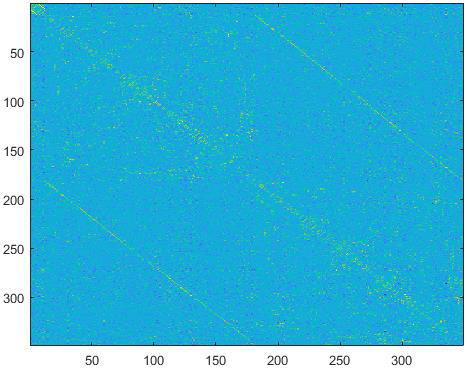
\includegraphics[scale=0.9]{appendix_scripts_and_figures/appendix_one_file_per_1.png}
	\caption{ }
	\label{fig:appendix_one_file_per_1}
\end{figure} \

\textbf{Script:}

\lstinputlisting{appendix_scripts_and_figures/script_create_one_file_per_row.m}


\section{Compute atlas for connectivity matrix}

In order to build connectivity matrices based on time series extracted from a brain parcellation, you first need to have a list of anatomical parcels, originating from some brain parcellation, and also to have each of them associated to a larger `network'.
\\

In the example here, there are 349 anatomical parcels with their characteristics (columns A through F) and their names (column G), and they are all associated to larger `networks' (column H). You then need to save your file in a .csv (or an Excel) file.

\begin{figure}[!h]
	\centering
		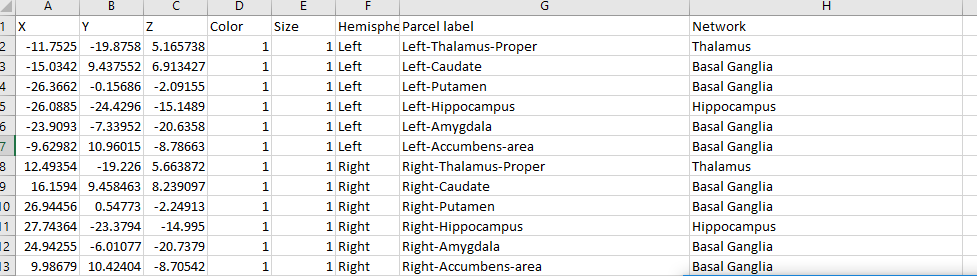
\includegraphics[scale=0.8]{appendix_scripts_and_figures/appendix_compute_atlas_for_connectivity_1.png}
	\caption{ }
	\label{fig:appendix_compute_atlas_for_connectivity_1}
\end{figure}

This file is then loaded in Matlab (double-clicking or `uiopen') as a cell array. \textbf{Note:} Be careful to modify the `Output Type' field whenever needed.

\begin{figure}[!h]
	\centering
		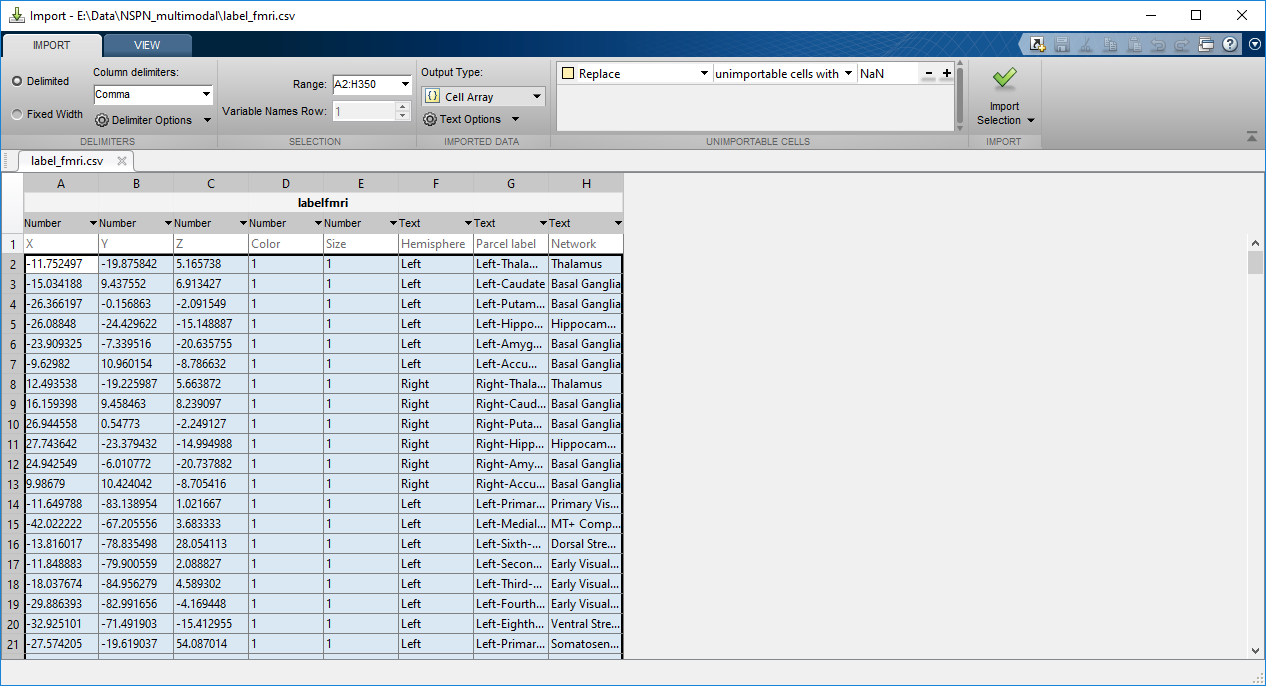
\includegraphics[scale=0.6]{appendix_scripts_and_figures/appendix_compute_atlas_for_connectivity_2.png}
	\caption{ }
	\label{fig:appendix_compute_atlas_for_connectivity_2}
\end{figure}

The last column of the cell array will then represent the `network' each time series belongs to. The variable name of the whole cell array in this example is `labelfmri', and it is only the last column ($labelfmri(:,end)$) containing the `networks' that you need to pass to the script.
\\

$\>> [atl\_mat,ROI\_names] = script\_build\_atlas\_from\_cell\_array(labelfmri(:,end));$
\\

This outputs and saves the atlas file and its corresponding labels for use in PRoNTo. \textbf{Note:} Please ensure to rename both of these files if you need to create multiple atlases (otherwise they will be over-written).
\\

The atlas is a 2D matrix of size 349*349 that contains an integer for each ‘network i – network j’ interaction. Here, 25 `networks' were defined, giving 325 pairwise interactions (n*(n-1)/2, with n the number of networks). The matrix is upper diagonal to ensure to mask out redundant features (as correlations are undirected). \textbf{Note:} For directed interactions, the full matrix would need to be generated (and the script to be modified).
\\[1cm]

\begin{figure}[!h]
	\centering
		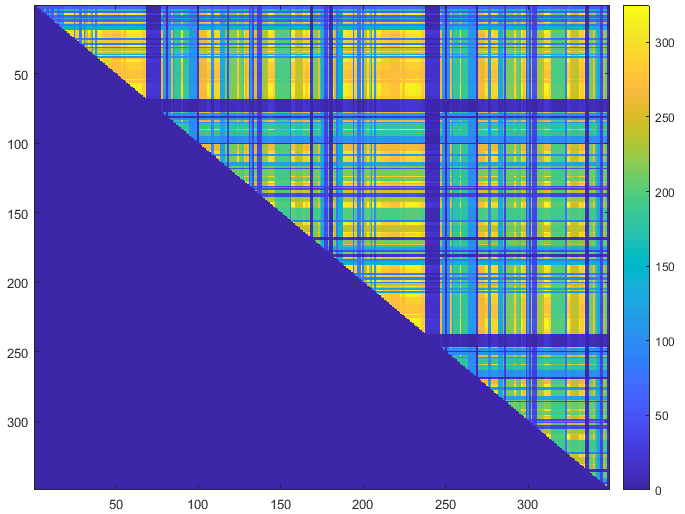
\includegraphics[scale=0.7]{appendix_scripts_and_figures/appendix_compute_atlas_for_connectivity_3.png}
	\caption{ }
	\label{fig:appendix_compute_atlas_for_connectivity_3}
\end{figure}

\textbf{Script:}
\\

\lstinputlisting{appendix_scripts_and_figures/script_build_atlas_from_cell_array.m}

\section{Connectivity matrix from MEEG}

Below is a script provided, if one wants to create a connectivity matrix from averaged EEG or MEG trials (here both). The script as it is, goes through all the subjects of the Multimodal SPM dataset, computes correlations between all variables and creates the connectivity matrix, which is then saved inside each subject's folder. These connectivity matrices created by this script are also the ones we use in the tutorial. In order for this script to run, you only need to modify the `prepath' accordingly.
\\

\lstinputlisting{appendix_scripts_and_figures/connectivity_matrix_from_MEEG.m} \


Alternatively, the matrices can be saved as 2D arrays instead of taking only the upper triangular part (remove line `\textit{conn\_mat = conn\_mat(mask)}'). In this case, a second-level mask should however be provided (save the defined mask in a separate file, i.e. \textit{save( mask.mat', `mask')}).


\section{Connectivity ROI weights}

The reader is referred to \ref{ssec:atlas_w_mat} for information related to the use of these scripts. In order for thesee scripts to run, you only need to modify the `prepath' accordingly.
\\

\textbf{Script 1:} Gather the atlas information (hard-coded here) and compute a summarized `network' matrix (i.e. \#networks x \#networks instead of \#channels x \#channels).
\\

\lstinputlisting{appendix_scripts_and_figures/connectivity_ROI_weights_1.m}  \

\textbf{Script 2:} Plot schemaball of kernel contributions from a symmetric 2D matrix (first input), the network labels (a cell array, 2nd input), the colormap to plot the curves in (3rd input) and the color of the nodes to represent within-network contributions (4th input). This code was modified from the schemaball.m written by Oleg Komarov found on Matlab’s file exchange.
\\

\lstinputlisting{appendix_scripts_and_figures/schemaball_JS.m}































